\subsection{Procesos psicrométricos}

    \begin{figure}[h]
        \centering
        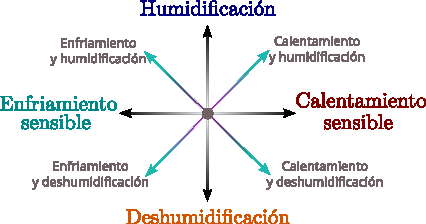
\includegraphics[width=0.4\textwidth, angle=0]{resources/images/vectorial/Psychrometry_Process.pdf}
        \caption{ ($x=1$).}
    \end{figure}
        


    \subsubsection{Calentamiento y Enfriamiento sensible}
        % Es la energía requerida para incrementar la temperatura de un material sin un cambio de fase
        Se refiere a la adición o eliminación de calor sin un cambio en el contenido de humedad; pero si en el cambio de la temperatura de bulbo seco lo que significa que cambia la humedad relativa. El punto de estado actual se moverá horizontalmente hacia la izquierda (enfriamiento) o hacia la derecha(calentamiento).
    
    \subsubsection{Deshumidificación por enfriamiento}
        La dehumidification a través del proceso de enfriamiento (desplazamiento hacia la izquierda) la linea de saturación, el vapor comienza a condesarse (a la temperatura de punto de rocío) y continua con la condensación a lo largo de la linea de saturación y disminuyendo su temperatura de rocío.
        
    \subsubsection{Humidificación y deshumidificación}
        %
    \subsubsection{Humidificación y deshumidificación}
        %

    \subsubsection{Enfriamiento y humidificación adiabática}
        %

    \subsubsection{Enfriamiento y humidificación por inyección de agua}
        %

    \subsubsection{Calentamiento y humidificación}
        %

    \subsubsection{Humidificación por inyección de vapor}
        %

    \subsubsection{Deshumidificación química adiabática}
        %

    \subsubsection{Mezcla adiabática de corrientes de aire}
        %
